\documentclass[8pt]{beamer}

% Beamer style
%\usetheme[secheader]{Madrid}
% \usetheme{CambridgeUS}
\useoutertheme{infolines}
\usecolortheme[rgb={0.65,0.15,0.25}]{structure}
% \usefonttheme[onlymath]{serif}
\beamertemplatenavigationsymbolsempty
%\AtBeginSubsection

% Packages
%\usepackage[french]{babel}
\usepackage[latin1]{inputenc}
\usepackage{color}
% \usepackage[dvipsnames]{xcolor}
\usepackage{xspace}
\usepackage{dsfont, stmaryrd}
\usepackage{amsmath, amsfonts, amssymb, stmaryrd, mathabx}
\usepackage{epsfig}
\usepackage{tikz}
\usepackage{url}
\usepackage{array}
\usepackage{/home/robin/LATEX/Biblio/astats}
%\usepackage[all]{xy}
\usepackage{graphicx}

% Maths
% \newtheorem{theorem}{Theorem}
% \newtheorem{definition}{Definition}
\newtheorem{proposition}{Proposition}
% \newtheorem{assumption}{Assumption}
% \newtheorem{algorithm}{Algorithm}
% \newtheorem{lemma}{Lemma}
% \newtheorem{remark}{Remark}
% \newtheorem{exercise}{Exercise}
% \newcommand{\propname}{Prop.}
% \newcommand{\proof}{\noindent{\sl Proof:}\quad}
% \newcommand{\eproof}{$\blacksquare$}

% \setcounter{secnumdepth}{3}
% \setcounter{tocdepth}{3}
\newcommand{\pref}[1]{\ref{#1} p.\pageref{#1}}
\newcommand{\qref}[1]{\eqref{#1} p.\pageref{#1}}

% Colors : http://latexcolor.com/
\definecolor{darkred}{rgb}{0.65,0.15,0.25}
\definecolor{darkgreen}{rgb}{0,0.4,0}
\definecolor{darkred}{rgb}{0.65,0.15,0.25}
\definecolor{amethyst}{rgb}{0.6, 0.4, 0.8}
\definecolor{asparagus}{rgb}{0.53, 0.66, 0.42}
\definecolor{applegreen}{rgb}{0.55, 0.71, 0.0}
\definecolor{awesome}{rgb}{1.0, 0.13, 0.32}
\definecolor{blue-green}{rgb}{0.0, 0.87, 0.87}
\definecolor{red-ggplot}{rgb}{0.52, 0.25, 0.23}
\definecolor{green-ggplot}{rgb}{0.42, 0.58, 0.00}
\definecolor{purple-ggplot}{rgb}{0.34, 0.21, 0.44}
\definecolor{blue-ggplot}{rgb}{0.00, 0.49, 0.51}

% Commands
\newcommand{\backupbegin}{
   \newcounter{finalframe}
   \setcounter{finalframe}{\value{framenumber}}
}
\newcommand{\backupend}{
   \setcounter{framenumber}{\value{finalframe}}
}
\newcommand{\emphase}[1]{\textcolor{darkred}{#1}}
\newcommand{\comment}[1]{\textcolor{gray}{#1}}
\newcommand{\paragraph}[1]{\textcolor{darkred}{#1}}
\newcommand{\refer}[1]{{\small{\textcolor{gray}{{\cite{#1}}}}}}
\newcommand{\Refer}[1]{{\small{\textcolor{gray}{{[#1]}}}}}
\newcommand{\goto}[1]{{\small{\textcolor{blue}{[\#\ref{#1}]}}}}
\renewcommand{\newblock}{}

\newcommand{\tabequation}[1]{{\medskip \centerline{#1} \medskip}}
% \renewcommand{\binom}[2]{{\left(\begin{array}{c} #1 \\ #2 \end{array}\right)}}

% Variables 
\newcommand{\Abf}{{\bf A}}
\newcommand{\Beta}{\text{B}}
\newcommand{\Bcal}{\mathcal{B}}
\newcommand{\Bias}{\xspace\mathbb B}
\newcommand{\Cor}{{\mathbb C}\text{or}}
\newcommand{\Cov}{{\mathbb C}\text{ov}}
\newcommand{\cl}{\text{\it c}\ell}
\newcommand{\Ccal}{\mathcal{C}}
\newcommand{\cst}{\text{cst}}
\newcommand{\Dcal}{\mathcal{D}}
\newcommand{\Ecal}{\mathcal{E}}
\newcommand{\Esp}{\xspace\mathbb E}
\newcommand{\Espt}{\widetilde{\Esp}}
\newcommand{\Covt}{\widetilde{\Cov}}
\newcommand{\Ibb}{\mathbb I}
\newcommand{\Fcal}{\mathcal{F}}
\newcommand{\Gcal}{\mathcal{G}}
\newcommand{\Gam}{\mathcal{G}\text{am}}
\newcommand{\Hcal}{\mathcal{H}}
\newcommand{\Jcal}{\mathcal{J}}
\newcommand{\Lcal}{\mathcal{L}}
\newcommand{\Mt}{\widetilde{M}}
\newcommand{\mt}{\widetilde{m}}
\newcommand{\Nbb}{\mathbb{N}}
\newcommand{\Mcal}{\mathcal{M}}
\newcommand{\Ncal}{\mathcal{N}}
\newcommand{\Ocal}{\mathcal{O}}
\newcommand{\pt}{\widetilde{p}}
\newcommand{\Pt}{\widetilde{P}}
\newcommand{\Pbb}{\mathbb{P}}
\newcommand{\Pcal}{\mathcal{P}}
\newcommand{\Qcal}{\mathcal{Q}}
\newcommand{\qt}{\widetilde{q}}
\newcommand{\Rbb}{\mathbb{R}}
\newcommand{\Sbb}{\mathbb{S}}
\newcommand{\Scal}{\mathcal{S}}
\newcommand{\st}{\widetilde{s}}
\newcommand{\St}{\widetilde{S}}
\newcommand{\Tcal}{\mathcal{T}}
\newcommand{\todo}{\textcolor{red}{TO DO}}
\newcommand{\Ucal}{\mathcal{U}}
\newcommand{\Un}{\math{1}}
\newcommand{\Vcal}{\mathcal{V}}
\newcommand{\Var}{\mathbb V}
\newcommand{\Vart}{\widetilde{\Var}}
\newcommand{\Zcal}{\mathcal{Z}}

% Symboles & notations
\newcommand\independent{\protect\mathpalette{\protect\independenT}{\perp}}\def\independenT#1#2{\mathrel{\rlap{$#1#2$}\mkern2mu{#1#2}}} 
\renewcommand{\d}{\text{\xspace d}}
\newcommand{\gv}{\mid}
\newcommand{\ggv}{\, \| \, }
% \newcommand{\diag}{\text{diag}}
\newcommand{\card}[1]{\text{card}\left(#1\right)}
\newcommand{\trace}[1]{\text{tr}\left(#1\right)}
\newcommand{\matr}[1]{\boldsymbol{#1}}
\newcommand{\matrbf}[1]{\mathbf{#1}}
\newcommand{\vect}[1]{\matr{#1}} %% un peu inutile
\newcommand{\vectbf}[1]{\matrbf{#1}} %% un peu inutile
\newcommand{\trans}{\intercal}
\newcommand{\transpose}[1]{\matr{#1}^\trans}
\newcommand{\crossprod}[2]{\transpose{#1} \matr{#2}}
\newcommand{\tcrossprod}[2]{\matr{#1} \transpose{#2}}
\newcommand{\matprod}[2]{\matr{#1} \matr{#2}}
\DeclareMathOperator*{\argmin}{arg\,min}
\DeclareMathOperator*{\argmax}{arg\,max}
\DeclareMathOperator{\sign}{sign}
\DeclareMathOperator{\tr}{tr}
\newcommand{\ra}{\emphase{$\rightarrow$} \xspace}

% Hadamard, Kronecker and vec operators
\DeclareMathOperator{\Diag}{Diag} % matrix diagonal
\DeclareMathOperator{\diag}{diag} % vector diagonal
\DeclareMathOperator{\mtov}{vec} % matrix to vector
\newcommand{\kro}{\otimes} % Kronecker product
\newcommand{\had}{\odot}   % Hadamard product

% TikZ
\newcommand{\nodesize}{2em}
\newcommand{\edgeunit}{2.5*\nodesize}
\newcommand{\edgewidth}{1pt}
\tikzstyle{node}=[draw, circle, fill=black, minimum width=.75\nodesize, inner sep=0]
\tikzstyle{square}=[rectangle, draw]
\tikzstyle{param}=[draw, rectangle, fill=gray!50, minimum width=\nodesize, minimum height=\nodesize, inner sep=0]
\tikzstyle{hidden}=[draw, circle, fill=gray!50, minimum width=\nodesize, inner sep=0]
\tikzstyle{hiddenred}=[draw, circle, color=red, fill=gray!50, minimum width=\nodesize, inner sep=0]
\tikzstyle{observed}=[draw, circle, minimum width=\nodesize, inner sep=0]
\tikzstyle{observedred}=[draw, circle, minimum width=\nodesize, color=red, inner sep=0]
\tikzstyle{eliminated}=[draw, circle, minimum width=\nodesize, color=gray!50, inner sep=0]
\tikzstyle{empty}=[draw, circle, minimum width=\nodesize, color=white, inner sep=0]
\tikzstyle{blank}=[color=white]
\tikzstyle{nocircle}=[minimum width=\nodesize, inner sep=0]

\tikzstyle{edge}=[-, line width=\edgewidth]
\tikzstyle{edgebendleft}=[-, >=latex, line width=\edgewidth, bend left]
\tikzstyle{edgebendright}=[-, >=latex, line width=\edgewidth, bend right]
\tikzstyle{lightedge}=[-, line width=\edgewidth, color=gray!50]
\tikzstyle{lightedgebendleft}=[-, >=latex, line width=\edgewidth, bend left, color=gray!50]
\tikzstyle{lightedgebendright}=[-, >=latex, line width=\edgewidth, bend right, color=gray!50]
\tikzstyle{edgered}=[-, line width=\edgewidth, color=red]
\tikzstyle{edgebendleftred}=[-, >=latex, line width=\edgewidth, bend left, color=red]
\tikzstyle{edgebendrightred}=[-, >=latex, line width=\edgewidth, bend right, color=red]

\tikzstyle{arrow}=[->, >=latex, line width=\edgewidth]
\tikzstyle{arrowbendleft}=[->, >=latex, line width=\edgewidth, bend left]
\tikzstyle{arrowbendright}=[->, >=latex, line width=\edgewidth, bend right]
\tikzstyle{arrowred}=[->, >=latex, line width=\edgewidth, color=red]
\tikzstyle{arrowbendleftred}=[->, >=latex, line width=\edgewidth, bend left, color=red]
\tikzstyle{arrowbendrightred}=[->, >=latex, line width=\edgewidth, bend right, color=red]
\tikzstyle{arrowblue}=[->, >=latex, line width=\edgewidth, color=blue]
\tikzstyle{dashedarrow}=[->, >=latex, dashed, line width=\edgewidth]
\tikzstyle{dashededge}=[-, >=latex, dashed, line width=\edgewidth]
\tikzstyle{dashededgebendleft}=[-, >=latex, dashed, line width=\edgewidth, bend left]
\tikzstyle{lightarrow}=[->, >=latex, line width=\edgewidth, color=gray!50]

\newcommand{\dN}{\Delta N}
\newcommand{\dtau}{\Delta \tau}

% Directory
\newcommand{\figcp}{/home/robin/RECHERCHE/RUPTURES/EXPOSES/FIGURES}

%====================================================================
%====================================================================

%====================================================================
%====================================================================
\begin{document}
%====================================================================
%====================================================================

%====================================================================
\title[Segmentation/culstering in a Poisson process]{Change-point detection \& clustering in a Poisson process}

\author[S. Robin]{S. Robin \\ \medskip
joint ongoing work with E. Lebarbier, C. Dion-Blanc}

\institute[]{Sorbonne universit�}

\date[Rochebrune'24]{Stats au sommet, Rochebrune, Mar. 2024}

%====================================================================
%====================================================================
\maketitle

%====================================================================
%====================================================================
\section{Previously in Rochebrune}
%====================================================================
\frame{\frametitle{Previously in Rochebrune} 

  \begin{tabular}{cc}
    \hspace{-.04\textwidth}
    \begin{tabular}{p{.45\textwidth}}
      \onslide+<2->{
      \paragraph{Point process on $t \in [0, 1]$.} \\ ~\\
      Event times:
      $$
      0 < T_1 < \dots T_i < \dots T_n < 1
      $$ \\
      
      Counting process:
      $$
      N(t) = \sum_{i=1}^n \Ibb\{T_i \leq t\}
      $$}      
      
      \onslide+<3->{
      \bigskip
      \paragraph{Poisson Process.}
      $$
      \{N(t)\}_{0 \leq t \leq 1} \sim PP(\lambda(t))
      $$}
    \end{tabular}
    & 
    \hspace{-.05\textwidth}
    \begin{tabular}{p{.5\textwidth}}
      \begin{overprint}
        \onslide<1>
        \paragraph{Bat cries} \\ ~\\
        \includegraphics[width=.45\textwidth, trim=0 10 10 10, clip=]{\figcp/ChauveSouris-GrandBourg-NB}
        \onslide<2->
        \paragraph{Bat cries}\footnote{source: Vigie-Chiro program, Y. Bas, CESCO-MNHN} \\ 
        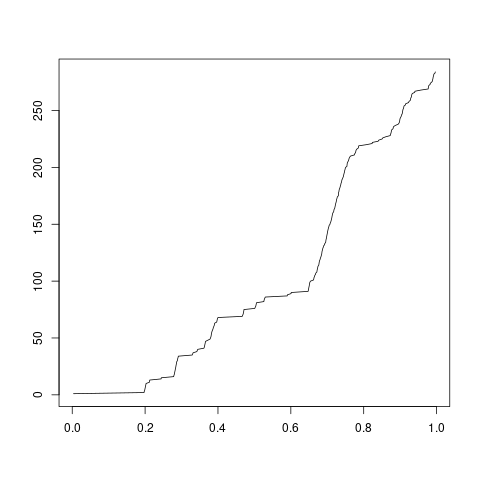
\includegraphics[width=.45\textwidth, trim=0 10 0 50, clip=]{\figcp/Chiro-sequence2295-path}
      \end{overprint}
    \end{tabular}
  \end{tabular}

  \bigskip
  \onslide+<3->{\paragraph{Intensity function $\lambda(t)$:} 
  $$
  \lambda(t) = \lim_{\Delta t \rightarrow 0} \frac{\Pbb\{N(t+\Delta t) - N(t) = 1\}}{\Delta t}, 
  \qquad \qquad 
  \Esp N(s) - \Esp N(t) = \int_t^s \lambda(u) \d u
  $$}
  
}

%====================================================================
\frame{\frametitle{Previously in Rochebrune} 

  \begin{tabular}{cc}
    \hspace{-.04\textwidth}
    \begin{tabular}{p{.45\textwidth}}
      \paragraph{Piecewise constant intensity function.} \\ ~ \\
      Change-points
      $$
      (\tau_0 =) 0 < \tau_1 \dots < \tau_{K-1} < 1 (= \tau_K)
      $$ \\
      
      For $t \in I_k = ]\tau_{k-1}, \tau_k]$:
      $$
      \lambda(t) = \lambda_k
      $$ \\
      
      \ra Continuous piece-wise linear cumulated intensity function      
    \end{tabular}
    & 
    \hspace{-.05\textwidth}
    \begin{tabular}{p{.45\textwidth}}
      \begin{overprint}
        \onslide<1>
        \paragraph{Bat cries}\footnote{source: Vigie-Chiro program, Y. Bas, CESCO-MNHN} \\
        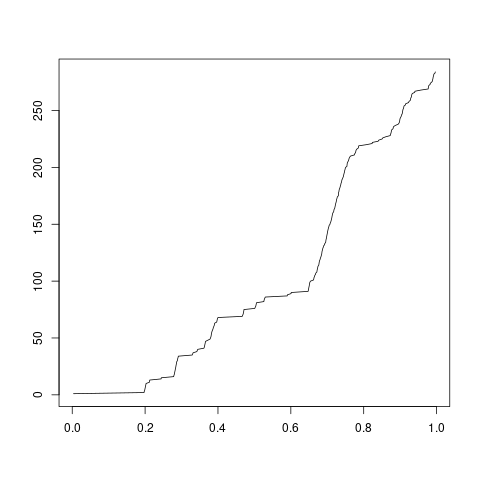
\includegraphics[width=.45\textwidth, trim=0 10 0 50, clip=]{\figcp/Chiro-sequence2295-path}
        \onslide<2>
        \paragraph{Bat cries}\footnote{source: Vigie-Chiro program, Y. Bas, CESCO-MNHN} \\
        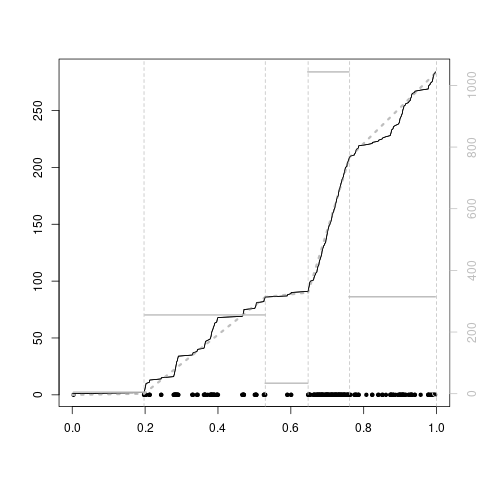
\includegraphics[width=.45\textwidth, trim=0 10 0 50, clip=]{\figcp/Chiro-sequence2295-K5-seg}
      \end{overprint}
    \end{tabular}
  \end{tabular}
  
  \pause
  \paragraph{Aim.} 
  \begin{itemize}
   \item Segmentation: estimate $(\tau, \lambda)$ reasonnably fast 
   \item Model selection: choose $K$
  \end{itemize}
}

%====================================================================
\frame{\frametitle{Previously in Rochebrune} 

  \begin{tabular}{cc}
    \hspace{-.04\textwidth}
    \begin{tabular}{p{.5\textwidth}}
      \paragraph{Efficient change-point detection.} 
      If the constrast (e.g. neg-log-likelihood) is \\ ~
      \begin{itemize}
        \setlength{\itemsep}{1.05\baselineskip}
        \item additive wrt the segments and 
        \item concave wrt the length of each segment,
      \end{itemize}
      ~ \\ ~ \\ ~ \\ 
    \end{tabular}
    & 
    \hspace{-.02\textwidth}
    \begin{tabular}{p{.5\textwidth}}
      \begin{overprint}
        \onslide<2>
        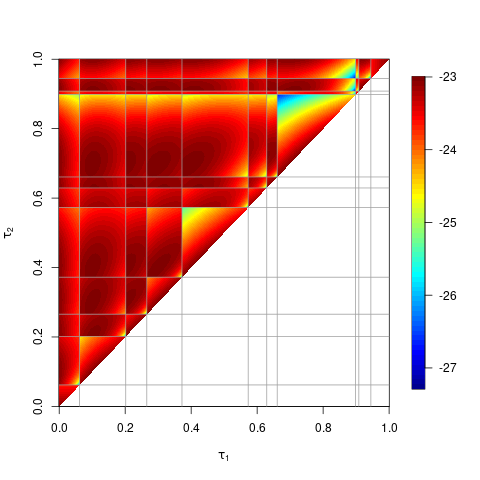
\includegraphics[width=.45\textwidth, trim=0 0 20 50, clip=]{\figcp/FigSegPP-simul-n10-K1-seed1-Contrast}  
        \onslide<3>
        \includegraphics[width=.385\textwidth, height=.30\textheight]{\figcp/Turtle-FriendsOfTheSea}        
        \onslide<4->
        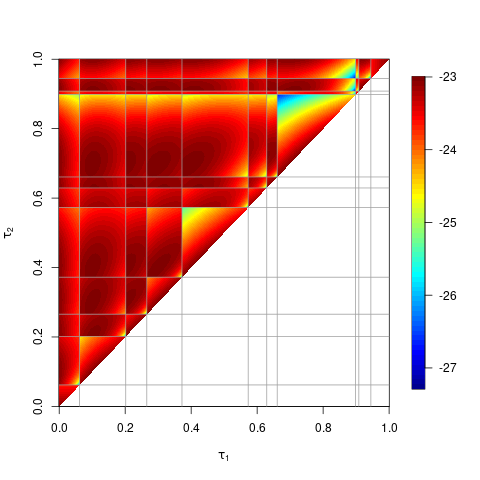
\includegraphics[width=.45\textwidth, trim=0 0 20 50, clip=]{\figcp/FigSegPP-simul-n10-K1-seed1-Contrast}  
      \end{overprint}
    \end{tabular}
  \end{tabular}
  
  \vspace{-.075\textheight}
  \onslide<5->{
  then the optimal change points belong to 
  $$
  \{T_1^-, T_1, T_2^-, T_2, \dots T_i^-, T_i, \dots, T_n^-, T_n\}
  $$
  
  \bigskip
  \ra Continuous to discrete optimization problem \\
  \ra Dynamic programming algorithm $= \Ocal(n^2)$.}

}

%====================================================================
\frame{\frametitle{Previously in Rochebrune} 

  \begin{tabular}{cc}
    \hspace{-.04\textwidth}
    \begin{tabular}{p{.5\textwidth}}
      \paragraph{Lazy model selection.} Thining property: \\ ~
      \begin{itemize}
        \setlength{\itemsep}{1.05\baselineskip}
        \item independent processes with proportional internsities and common change point;
        \item cross-validation procedure to choose $K$.
      \end{itemize}
    \end{tabular}
    & 
    \hspace{-.075\textwidth}
    \begin{tabular}{p{.5\textwidth}}
      \begin{overprint}
        \onslide<1>
        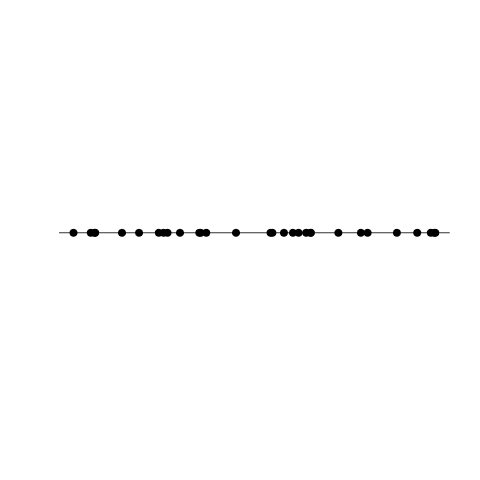
\includegraphics[width=.5\textwidth, trim=0 225 0 225, clip=]{\figcp/FigSegPP-ThiningOriginal.png} \\
        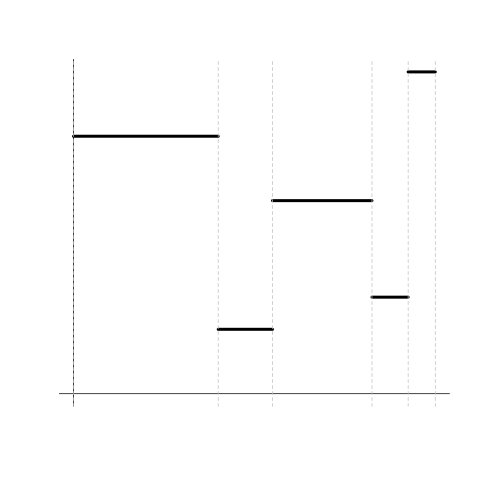
\includegraphics[width=.5\textwidth, height=.3\textheight, trim=0 0 0 0, clip=]{\figcp/FigSegPP-ThiningOriginalLambda.png}
        \onslide<2->
        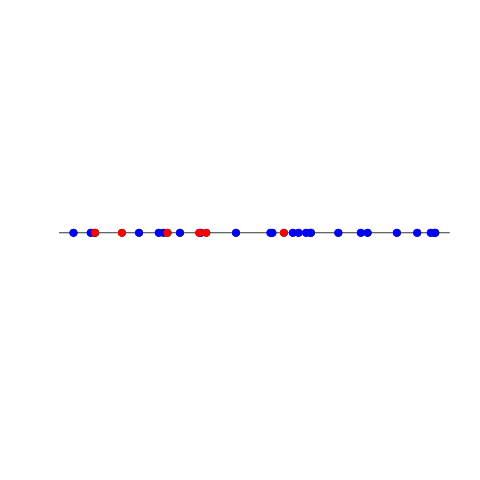
\includegraphics[width=.5\textwidth, trim=0 225 0 225, clip=]{\figcp/FigSegPP-ThiningSampling.png} \\
        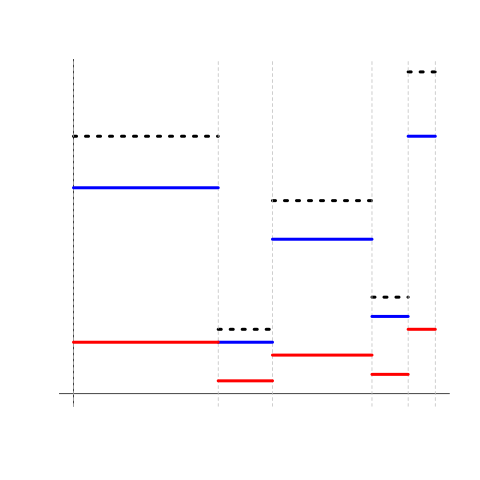
\includegraphics[width=.5\textwidth, height=.3\textheight, trim=0 0 0 0, clip=]{\figcp/FigSegPP-ThiningSamplingLambda.png}
      \end{overprint}
    \end{tabular}
  \end{tabular}
  \refer{DLR23}


  \bigskip \bigskip \pause
  \paragraph{On-going.} Consistency + (modified) BIC criterion for choosing $K$.
  
}

%====================================================================
%====================================================================
\section{Next step: clustering}
%====================================================================
\frame{\frametitle{Next step: clustering} 
  
  \begin{tabular}{cc}
    \hspace{-.04\textwidth}
    \begin{tabular}{p{.45\textwidth}}
      \onslide+<5->{
        \paragraph{Segment clustering.} $P$ groups of segments \\ ~
        \begin{itemize}
          \setlength{\itemsep}{1.05\baselineskip}
          \item each segments belong to one group 
          \item group = underlying behavior
        \end{itemize} 
        ~ \\~ \\
      }
    \end{tabular}
    & 
    \hspace{-.05\textwidth}
    \begin{tabular}{p{.5\textwidth}}
      \begin{overprint}
        \onslide<1>
%        \paragraph{Bat cries} \\ ~\\
        \includegraphics[width=.45\textwidth, trim=0 10 10 10, clip=]{\figcp/ChauveSouris-GrandBourg-NB}
        \onslide<2>
%        \paragraph{Bat cries} \\ ~\\
        \includegraphics[width=.45\textwidth, trim=0 10 10 10, clip=]{\figcp/ChauveSouris-GrandBourg}
        \onslide<3>
%        \paragraph{Bat cries}\footnote{source: Vigie-Chiro program, Y. Bas, CESCO-MNHN} \\ 
        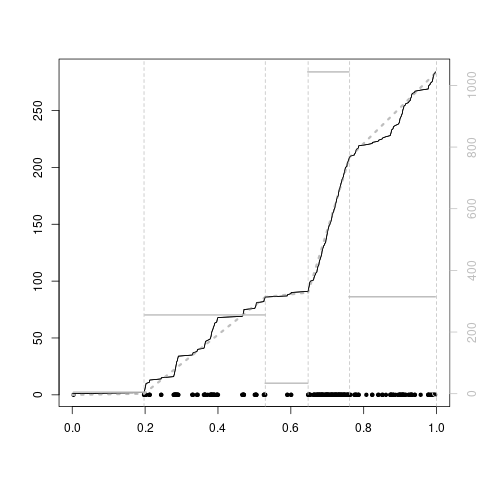
\includegraphics[width=.45\textwidth, trim=0 10 0 50, clip=]{\figcp/Chiro-sequence2295-K5-seg}
        \onslide<4->
%        \paragraph{Bat cries}\footnote{source: Vigie-Chiro program, Y. Bas, CESCO-MNHN} \\ 
        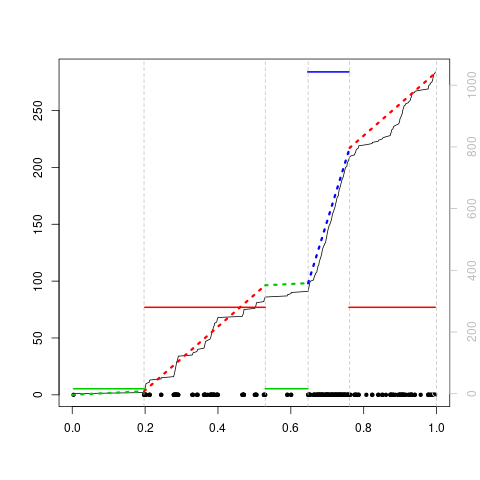
\includegraphics[width=.45\textwidth, trim=0 10 0 50, clip=]{\figcp/Chiro-sequence2295-K5-P3-segClassif}
      \end{overprint}
    \end{tabular}
  \end{tabular}

  
  \onslide+<6->{\vspace{-.15\textheight}\paragraph{Model.}
  \medskip
  \begin{itemize}
    \setlength{\itemsep}{1.05\baselineskip}
    \item $K$ segments $I_1, \dots I_K$
    \item Segment $k$ belongs to group $p$ with probability $\pi_p$
    \item Point process $N(I_k) \sim PP(\lambda_p)$
  \end{itemize}        
  }
}

%====================================================================
\frame{\frametitle{Segmentation-clustering model}

  \paragraph{More precisely.}
  \begin{itemize}
%     \setlength{\itemsep}{1.05\baselineskip}
    \item $K+1$ change-points: $\tau_0 = 0 < \tau_1 < \dots < \tau_{K-1} < \tau_K = 1$
    \item $K$ segments: $I_k = (\tau_{K-1}, \tau_K]$ 
    \item \pause $P$ groups, with proportions: $\pi = (\pi_1, \dots \pi_K)$
    \item $K$ latent variables (segment memberships):
    $$
    (Z_k)_{1 \leq k \leq K} \text{ iid} \sim \Mcal(1, \pi)
    $$
    \item \pause $P$ intensities: $\lambda = (\lambda_1, \dots \lambda_K)$
    \item Point process in segment $k$:
    $$
    N(Ik) \mid Z_k = p \sim PP(\lambda_p)
    $$
  \end{itemize}        
  
  \bigskip \pause
  \paragraph{Model parameters.}
  $$
  \theta = (\pi, \lambda, \tau)
  $$
  + $(K, P)$
}

%====================================================================
\frame{\frametitle{Inference algorithm (1/2)}

  \paragraph{Observed likelihood.} Segment $I_k = (\tau_{K-1}, \tau_K]$, width $\Delta \tau_k$, count $\Delta N_k$:
  $$
  \log p_\theta(N) 
  = \sum_{k=1}^K \log \left(\sum_{p=1}^P \pi_p p_{\lambda_p}(N(I_k))\right)
  = \sum_{k=1}^K \underset{\text{$-c(I_k)$}}{\underbrace{\log \left(\sum_{p=1}^P \pi_p e^{-\lambda_p \Delta \tau_k} \lambda_p^{\Delta N_k} \right)}}.
  $$
  
  \bigskip \pause 
  \begin{proposition}[concave constrast]
  The contrast $c(I_k)$ is a concave function of the width $\Delta \tau_k = \tau_{k} - \tau_{k-1}$ of interval $I_k$ 
  \end{proposition}

  \bigskip \bigskip \pause 
  \paragraph{Consequence.} For given mixture parameters $(\pi, \lambda)$, the optimal segmentation
  $$
  \widehat{\tau}(\pi, \lambda) = \argmax_\tau \log p_{(\pi, \lambda, \tau)}(N)
  $$
  is a subset of $\{T_1^-, T_1, T_2^-, T_2, \dots T_i^-, T_i, \dots, T_n^-, T_n\}$. 
}

%====================================================================
\frame{\frametitle{Inference algorithm (2/2)}

  \paragraph{Complete likelihood.} Denoting $Z_{kp} = \Ibb\{Z_k = p\}$,
  $$
  \log p_\theta(N, Z) = \sum_{k=1}^K \sum_{p=1}^P Z_{kp} \left(\log \pi_p + \log p_{\lambda_p}(N(I_k)) \right)
  $$
  
  \bigskip \bigskip \pause 
  \paragraph{'EM-DP' algorithm.} (see \refer{PRL07} for a discrete time version)
  \begin{description}
    \setlength{\itemsep}{1.1\baselineskip}
    \item[Clustering.] Given $\tau^{(h)}$, get
    $$
    (\pi, \lambda)^{(h+1)} = \argmax_{(\pi, \lambda)} \log p_{(\pi, \lambda, \tau^{(h)})}(N)
    $$
    using expectation-maximization (EM), based on $\Esp_\theta(\log p_\theta(N, Z) \mid N)$; 
    \item[Segmentation.] Given $(\pi^{(h+1)}, \lambda^{(h+1)})$, get
    $$
    \tau^{(h+1)} = \argmax_\tau \log p_{(\pi^{(h+1)}, \lambda^{(h+1)}, \tau)}(N)
    $$
    using dynamic programming (DP).
  \end{description}
  
}

%====================================================================
\frame{\frametitle{In practice}

  \begin{tabular}{cc}
    \hspace{-.04\textwidth}
    \begin{tabular}{p{.5\textwidth}}
      \begin{itemize}
        \setlength{\itemsep}{1.05\baselineskip}
        \item Need to run EM-DP for 
        $$
        1 \leq K \leq K_{\max}, \quad 1 \leq P \leq P_{\max}
        $$
      \item With few guaranty to attain the global optimum (very few EM iterations) 
      \item \onslide+<2->{Need for (time-consuming) smoothing steps, restarting EM-DP \\
      \ra with neighbor mixture parms: 
      \begin{align*}
        (\widehat{\pi}_{\emphase{K-1}, P}, \widehat{\lambda}_{\emphase{K-1}, P}, \widehat{\tau}_{K, P}) \\
        (\widehat{\pi}_{\emphase{K+1}, P}, \widehat{\lambda}_{\emphase{K+1}, P}, \widehat{\tau}_{K, P})
      \end{align*}
%       $$(\widehat{\pi}_{K-1, P}, \widehat{\lambda}_{K-1, P}, \widehat{\tau}_{K, P})$$
%       $$(\widehat{\pi}_{K+1, P}, \widehat{\lambda}_{K+1, P}, \widehat{\tau}_{K, P})$$
      \ra or neighbor segmentation parms: 
      \begin{align*}
      (\widehat{\pi}_{K, P}, \widehat{\lambda}_{K, P}, \widehat{\tau}_{K, \emphase{P-1}}) \\
      (\widehat{\pi}_{K, P}, \widehat{\lambda}_{K, P}, \widehat{\tau}_{K, \emphase{P+1}})
      \end{align*}
%       $$(\widehat{\pi}_{K, P}, \widehat{\lambda}_{K, P}, \widehat{\tau}_{K, P-1})$$
%       $$(\widehat{\pi}_{K, P}, \widehat{\lambda}_{K, P}, \widehat{\tau}_{K, P+1})$$
      }
      \end{itemize}
    \end{tabular}
    & 
    \hspace{-.05\textwidth}
    \begin{overprint}
      \onslide<1>
      \begin{tabular}{c}
        First rounds of EM-DP \\
        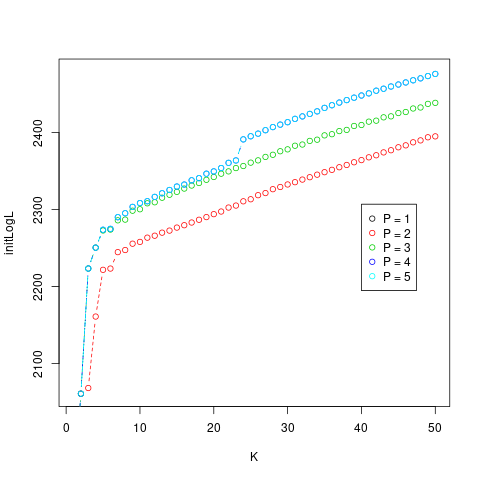
\includegraphics[width=.45\textwidth, trim=5 20 20 50, clip=]{\figcp/Chiro-sequence2147-logLpathInit}      
      \end{tabular}
      \onslide<2>
      \begin{tabular}{c}
        After smoothing \\
        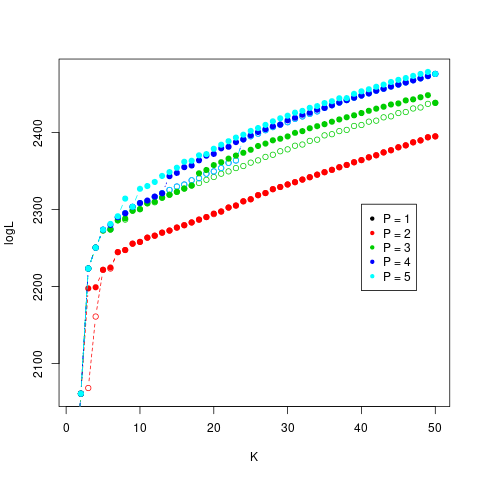
\includegraphics[width=.45\textwidth, trim=5 20 20 50, clip=]{\figcp/Chiro-sequence2147-logLpathImprove}      
      \end{tabular}
    \end{overprint}
  \end{tabular}

}

%====================================================================
\frame{\frametitle{Model selection}

  \begin{tabular}{cc}
    \hspace{-.04\textwidth}
    \begin{tabular}{p{.5\textwidth}}
      \begin{itemize}
        \setlength{\itemsep}{1.05\baselineskip}
        \item Need to select both $K$ and $P$
        \item Cross-validation too demanding
        \item \onslide+<2->{BIC penalty for mixture
        $$
        pen(P) = (2P - 1) \log(K)/2
        $$
         (wrong: see \refer{LeM06})}
        \item \onslide+<3->{Penalty for segmentation: slope heuristic (capushe)}
      \end{itemize}
      \\ ~ \\ ~ \\
    \end{tabular}
    & 
    \hspace{-.05\textwidth}
%     \begin{tabular}{c}
      \begin{overprint}
        \onslide<1>
        \begin{tabular}{c}
        $\log p_{K, P}(N)$ \\
        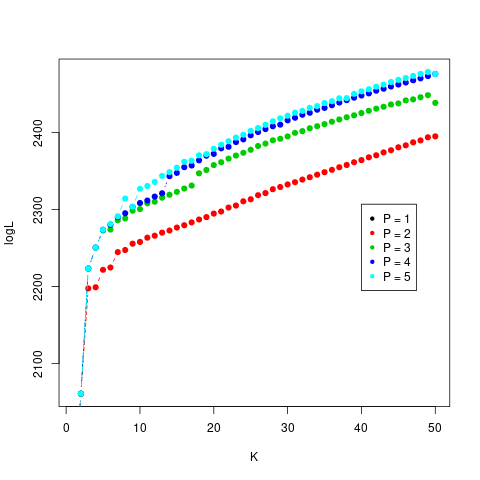
\includegraphics[width=.45\textwidth, trim=5 20 20 50, clip=]{\figcp/Chiro-sequence2147-logL}      
        \end{tabular}
        \onslide<2>
        \begin{tabular}{c}
        $BIC_{\text{mixture}}(K, P)$ \\
        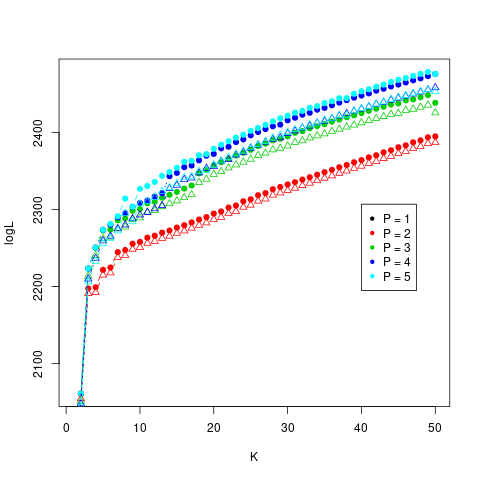
\includegraphics[width=.45\textwidth, trim=5 20 20 50, clip=]{\figcp/Chiro-sequence2147-BICmixture}      
        \end{tabular}
        \onslide<3>
        \begin{tabular}{c}
        $\widehat{K} = 13, \widehat{P} = 5$ \\
        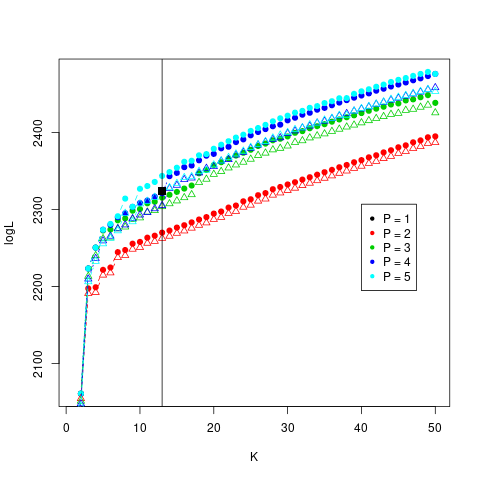
\includegraphics[width=.45\textwidth, trim=5 20 20 50, clip=]{\figcp/Chiro-sequence2147-select}      
        \end{tabular}
      \end{overprint}
%     \end{tabular}
  \end{tabular}

}

%====================================================================
%====================================================================
\section{Illustrations}
%====================================================================
\frame{\frametitle{Some examples}

  \newcommand{\seq}{2295} \newcommand{\Kdp}{16} \newcommand{\Kemdp}{14}
  \newcommand{\Pemdp}{3}
  \vspace{-.05\textheight}
  $$
  \begin{tabular}{m{.25\textwidth}m{.35\textwidth}m{.35\textwidth}}
    \begin{tabular}{p{.2\textwidth}}
      Segmentation \\ (DP)
    \end{tabular}
    & 
    \hspace{-0.1\textwidth}
    \begin{tabular}{c}
      $\widehat{K}_{DP} = \Kdp$ \\
      \includegraphics[width=.33\textwidth, trim=10 30 0 50, clip=]{\figcp/Chiro-sequence\seq-K\Kdp-seg}
    \end{tabular}
    & 
    \hspace{-0.1\textwidth}
    \begin{tabular}{c}
      $\widehat{K}_{EMDP} = \Kemdp$ \\
      \includegraphics[width=.33\textwidth, trim=10 30 0 50, clip=]{\figcp/Chiro-sequence\seq-K\Kemdp-seg}
    \end{tabular}
    \\
    \begin{tabular}{p{.2\textwidth}}
      Segmentation \\ clustering \\ (EM-DP)
    \end{tabular}
    &
    \hspace{-0.1\textwidth}
    \begin{tabular}{c}
      $\widehat{K}_{DP} = \Kdp$, $\widehat{P}_{EMDP} = \Pemdp$ \\
      \includegraphics[width=.33\textwidth, trim=10 30 0 50, clip=]{\figcp/Chiro-sequence\seq-K\Kdp-P\Pemdp-segClassif}
    \end{tabular}
    & 
    \hspace{-0.1\textwidth}
    \begin{tabular}{c}
      $\widehat{K}_{EMDP} = \Kemdp$, $\widehat{P}_{EMDP} = \Pemdp$ \\
      \includegraphics[width=.33\textwidth, trim=10 30 0 50, clip=]{\figcp/Chiro-sequence\seq-K\Kemdp-P\Pemdp-segClassif}
    \end{tabular}
  \end{tabular}
  $$
}

%====================================================================
\frame{\frametitle{Some examples}

  \newcommand{\seq}{1082} \newcommand{\Kdp}{7} \newcommand{\Kemdp}{23}
  \newcommand{\Pemdp}{5}
  \vspace{-.05\textheight}
  $$
  \begin{tabular}{m{.25\textwidth}m{.35\textwidth}m{.35\textwidth}}
    \begin{tabular}{p{.2\textwidth}}
      Segmentation \\ (DP)
    \end{tabular}
    & 
    \hspace{-0.1\textwidth}
    \begin{tabular}{c}
      $\widehat{K}_{DP} = \Kdp$ \\
      \includegraphics[width=.33\textwidth, trim=10 30 0 50, clip=]{\figcp/Chiro-sequence\seq-K\Kdp-seg}
    \end{tabular}
    & 
    \hspace{-0.1\textwidth}
    \begin{tabular}{c}
      $\widehat{K}_{EMDP} = \Kemdp$ \\
      \includegraphics[width=.33\textwidth, trim=10 30 0 50, clip=]{\figcp/Chiro-sequence\seq-K\Kemdp-seg}
    \end{tabular}
    \\
    \begin{tabular}{p{.2\textwidth}}
      Segmentation \\ clustering \\ (EM-DP)
    \end{tabular}
    &
    \hspace{-0.1\textwidth}
    \begin{tabular}{c}
      $\widehat{K}_{DP} = \Kdp$, $\widehat{P}_{EMDP} = \Pemdp$ \\
      \includegraphics[width=.33\textwidth, trim=10 30 0 50, clip=]{\figcp/Chiro-sequence\seq-K\Kdp-P\Pemdp-segClassif}
    \end{tabular}
    & 
    \hspace{-0.1\textwidth}
    \begin{tabular}{c}
      $\widehat{K}_{EMDP} = \Kemdp$, $\widehat{P}_{EMDP} = \Pemdp$ \\
      \includegraphics[width=.33\textwidth, trim=10 30 0 50, clip=]{\figcp/Chiro-sequence\seq-K\Kemdp-P\Pemdp-segClassif}
    \end{tabular}
  \end{tabular}
  $$
}

%====================================================================
%====================================================================
\section{Conclusion}
%====================================================================
\frame{\frametitle{To summarize (1/2)}

  Segmentation-clustering allows to classify segment according to underlying behaviors

  \bigskip \bigskip \pause
  \paragraph{What does work.} \\ ~
  \begin{itemize}
    \setlength{\itemsep}{1.05\baselineskip}
    \item Segmentation step still efficient thank to the concavity property
    \item Fast (!) EM-DP algorithm for the whole inference
  \end{itemize}

  \bigskip \bigskip \pause
  \paragraph{What does not work.} \\ ~
  \begin{itemize}
    \setlength{\itemsep}{1.05\baselineskip}
    \item Exploration of $(K, P)$ computationaly demanding
    \item Need for a dedicated model selection procedure
  \end{itemize}

}

%====================================================================
\frame{\frametitle{To summarize (2/2)}

$$
\text{\Large effici\textcolor{red}{E}nt c\textcolor{red}{L}ustering and seg\textcolor{red}{ME}ntation of Poisson p\textcolor{red}{R}ocesses}
$$
\pause
$$
\begin{tabular}{m{.4\textwidth}m{.1\textwidth}m{.4\textwidth}}
%   segmentation & & segmentation / clustering \\
  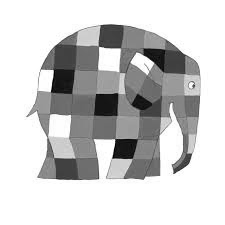
\includegraphics[width=.35\textwidth, trim=5 5 5 5, clip=]{\figcp/Elmer-NB}
  & $\longrightarrow$
  & 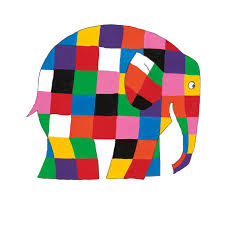
\includegraphics[width=.35\textwidth, trim=5 5 5 5, clip=]{\figcp/Elmer}
\end{tabular}
$$
}

%====================================================================
\frame{ \frametitle{References}
  {
   \footnotesize
   \bibliography{/home/robin/Biblio/BibGene}
   \bibliographystyle{alpha}
  }
}

%====================================================================
\backupbegin
%====================================================================


%====================================================================
\backupend
%====================================================================

%====================================================================
%====================================================================
\end{document}
%====================================================================
%====================================================================
  
  \begin{tabular}{cc}
    \hspace{-.04\textwidth}
    \begin{tabular}{p{.5\textwidth}}
    \end{tabular}
    & 
    \hspace{-.02\textwidth}
    \begin{tabular}{p{.5\textwidth}}
    \end{tabular}
  \end{tabular}
